\chapter{Cuestionario} \label{Ap:cuestionario}

% the code below specifies where the figures are stored
\ifpdf
    \graphicspath{{Apendice/figures/PNG/}{Apendice/figures/PDF/}{Apendice/figures/}}
\else
    \graphicspath{{Apendice/figures/EPS/}{Apendice/figures/}}
\fi



\global\mdfdefinestyle{cuestionarioST}{%
linecolor=blue,linewidth=2pt,%
leftmargin=1cm,rightmargin=1cm
}

\global\mdfdefinestyle{hipotesis0}{%
linecolor=black,linewidth=1pt,%
leftmargin=1cm,rightmargin=1cm
}
Este apéndice contiene el cuestionario utilizado para el caso de la extracción de indicadores del wiki de Moodle con EvalCourse y un exhaustivo análisis de las respuestas recogidas. En concreto, las secciones de este apéndice son:

\begin{itemize}
	\item Cuestionario (ver sección~\ref{apc:sec:cuestionario})
	\item Resultados  (ver sección~\ref{apc:sec:resultados})
\end{itemize}

\newpage

\section{Cuestionario} \label{apc:sec:cuestionario}
	
	\subsection*{A. Nivel educativo}

\begin{mdframed}[style=cuestionarioST]
		Indique el nivel educativo en el que imparte su docencia:
			\begin{itemize}
				\item Infantil
				\item Primaria
				\item Secundaria
				\item Superior
				\item Otras
			\end{itemize}
\end{mdframed}

	\subsection*{B. Conocimientos de programación}

\begin{mdframed}[style=cuestionarioST]
			Indique los conocimientos de programación que considera que posee:
			\begin{itemize}
				\item Nulos
				\item Muy básicos
				\item Básicos
				\item Medios/avanzados
			\end{itemize}
\end{mdframed}

	
	%EvalCourse es un programa que mediante una consulta nos ofrece indicadores del trabajo de los estudiantes en el Wiki.

	\subsection*{C. Consultas de indicadores}

\begin{mdframed}[style=cuestionarioST]
	Se muestran dos consultas y las figuras obtenidas mediante EvalCourse. Los tres estudiantes que se mencionan trabajaron en una página del wiki entre las semanas 38 y 50 del curso, momento en que el trabajo debía estar terminado.
\end{mdframed}

\newpage

	\paragraph*{C.1 Consulta de indicadores 1}

\begin{mdframed}[style=cuestionarioST]
			A la vista de la figura~\ref{fig:SantaPie} obtenida con la consulta~\ref{code:apconsulta1}: ¿Sería capaz de valorar si los tres estudiantes han participado activamente en el wiki?
			\begin{itemize}
				\item Sí
				\item No
			\end{itemize}

			\rule{30mm}{1pt} \newline
\begin{lstlisting}[caption=Consulta participación de los estudiantes en el wiki,label=code:apconsulta1, captionpos=b, morekeywords={Evidence,get, students, show, milestones, participation, access, in, assignment, forum, campus, wiki, between, and, workshop, interaction, assessment, grade, from, course, backup}]
Evidence Participacion: 
	get students 
	show participation 
	in wiki.
\end{lstlisting}
\end{mdframed}

\begin{figure}[h]
 \begin{center}
    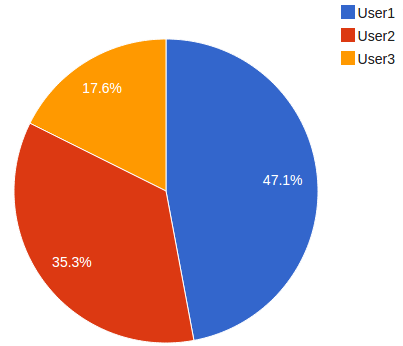
\includegraphics[scale=0.65]{santa_pie.png}
  \end{center}
  \caption{Participación de los estudiantes a la página del wiki}
  \label{fig:SantaPie}
\end{figure}

\newpage

%		\subsection*{Contribuciones aportadas por los estudiantes a lo largo del curso a la página del wiki}




%		\subsection*{Evolución del contenido aportado por los estudiantes a su página del wiki}

	\paragraph*{C.2 Consulta de indicadores 2}

\begin{mdframed}[style=cuestionarioST]

			A la vista de las figuras~\ref{fig:SantaContribuciones} y~\ref{fig:SantaEvolucion} obtenidos mediante la consulta~\ref{code:apconsulta2}: ¿Sería capaz de valorar si los estudiantes contribuyeron al wiki de forma contínua?
			\begin{itemize}
				\item Sí
				\item No
			\end{itemize}

			\rule{30mm}{1pt} \newline

\begin{lstlisting}[caption=Consulta participación de los estudiantes en el wiki,label=code:apconsulta2, captionpos=b, morekeywords={Evidence,get, students, show, milestones, participation, access, in, assignment, forum, campus, wiki, between, and, workshop, interaction, assessment, grade, from, course, backup}]
Evidence Contribuciones: 
	get students 
	show interaction 
	in wiki.
\end{lstlisting}
\end{mdframed}

\begin{figure}[h]
  \begin{center}
    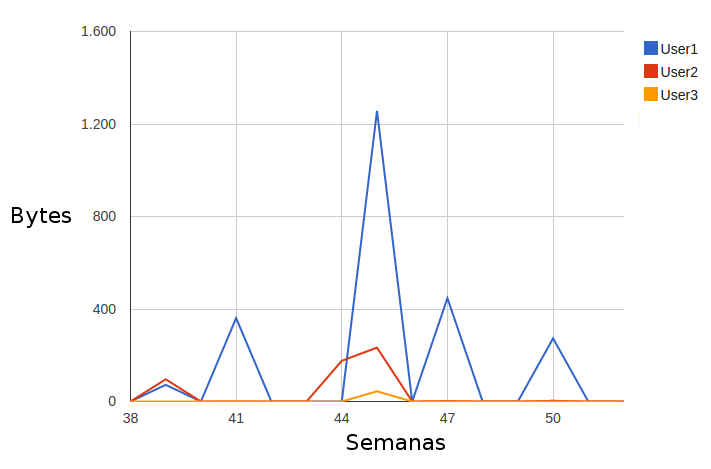
\includegraphics[scale=0.5]{santa_contribuciones.png}
  \end{center}
  \caption{Contribuciones de los estudiantes a la página del wiki}
  \label{fig:SantaContribuciones}
\end{figure}

\newpage

\begin{figure}[h]
  \begin{center}
    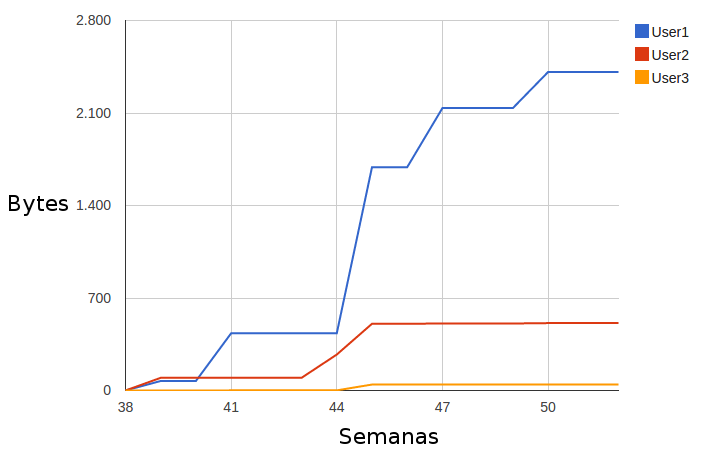
\includegraphics[scale=0.5]{santa_evolution.png}
  \end{center}
  \caption{Evolución del contenido de una página del wiki}
  \label{fig:SantaEvolucion}
\end{figure}

	\subsection*{D. Competencias evaluables}

\begin{mdframed}[style=cuestionarioST]
			Indique para evaluar qué competencias serían de utilidad los gráficos generados anteriormente.

			\rule{30mm}{1pt} \newline			

			Competencia de trabajo en equipo:
			\begin{itemize}
				\item Sí
				\item No
			\end{itemize}

			¿Por qué? \newline
			Explique por qué considera que sí o no sería posible evaluar la competencia de trabajo en equipo en el wiki a partir de los gráficos anteriores:\newline
			\rule{120mm}{1pt} \newline
			\rule{120mm}{1pt} \newline
			\bigskip

			Competencia de planificación y gestión del tiempo:
			\begin{itemize}
				\item Sí
				\item No
			\end{itemize}

			¿Por qué? \newline
			Explique por qué considera que sí o no sería posible evaluar la competencia de planificación y gestión del tiempo en el wiki a partir de los gráficos anteriores:\newline
			\rule{120mm}{1pt} \newline
			\rule{120mm}{1pt} \newline
			\bigskip

			Competencia de liderazgo
			\begin{itemize}
				\item Sí
				\item No
			\end{itemize}

			¿Por qué? \newline
			Explique por qué considera que sí o no sería posible evaluar la competencia de liderazgo en el wiki a partir de los gráficos anteriores:\newline
			\rule{120mm}{1pt} \newline
			\rule{120mm}{1pt} \newline
\end{mdframed}

\newpage

\section{Resultados} \label{apc:sec:resultados}

En esta sección se muestran y analizan en detalle los resultados del cuestionario. %Los comentarios sobre los resultados de los profesores se muestran en el capítulo X (esto se dice en la tesis de la uoc, tendré que ver qué comento yo).

\subsection{Poblaciones}

En este cuestionario participaron cuatro tipos de poblaciones. A cada una de ellas se le ha presentado el método DBA y la herramienta EvalCourse en un contexto diferente y con un nivel de detalle diferente, impuesto este por el foro en el que se presentaba. A continuación se presentan cada una de estas poblaciones y el feedback con el que respondieron el cuestionario.

\subsubsection{Curso innovación docente}
Profesorado de la Universidad de Cádiz que participó en el curso de innovación docente sobre wikis.
	\begin{itemize}
		\item{Forma de presentación:} Curso presencial.

		\item{Organización:} Dos sesiones de 4 horas cada una en la que se explicaba cómo trabajar en clase con wikis, se propusieron enfoques para favorecer el desempeño de competencias genéricas de los estudiantes y se presentaba el método DBA y la herramienta EvalCourse.  Además, se incluyeron actividades prácticas que se desarrollaron en las mismas sesiones.

		\item{Número de participantes:} 11
	\end{itemize}

\subsubsection{Taller Aulablog}
Profesorado a nivel nacional que asistió al taller sobre wikis en educación que se presentó en el encuentro de profesorado Aulablog 2015.

	\begin{itemize}
		\item{Forma de presentación:} Taller presencial.

		\item{Organización:} Una sesión de 3 horas en la que se explicó cómo trabajar en clase con wikis, se proponían enfoques para favorecer el desempeño de competencias genéricas de los estudiantes y se presentaba el método DBA y la herramienta EvalCourse.

		\item{Número de participantes:} 14
	\end{itemize}

\subsubsection{Actuación avalada}
Profesorado de la Universidad de Cádiz que participó en la actuación avalada sobre el uso de wikis.

	\begin{itemize}
		\item{Forma de presentación:} Entrevista personal.

		\item{Organización:} Se explicó a los participantes el método DBA y se les invitó a utilizar actividades en sus cursos virtuales que favoreciesen la actividad de los estudiantes en el curso para aplicar después EvalCourse. Se hizo especial hincapié en la inclusión de wikis en sus cursos virtuales. 

		\item{Número de participantes:} 7
	\end{itemize}

\subsubsection{MediaWiki}
Miembros de MediaWiki España que fueron invitados y aceptaron participar en el cuestionario.

	\begin{itemize}
		\item{Forma de presentación:} Correo electrónico.

		\item{Organización:} Mediante correo electrónico enviado a los miembros de MediaWiki España, se les explica el método DBA, la herramienta EvalCourse y se les invita a completar el cuestionario.

		\item{Número de participantes:} 19 % 1 de ellos no es mediawiki es L.Anido
	\end{itemize}

En total son 51 cuestionarios completados, repartidos tal y cómo se resume en la tabla~\ref{tab:ap:poblaciones:barras}.

\begin{table}
  \begin{center}
  \begin{tabular}{| m{5cm} | c | c |}
    \hline
    POBLACIÓN & CUESTIONARIOS & PORCENTAJE \\
    \hline
    \hline
    Curso innovación docente & 11 & 21,57\percentage \\
    \hline
    Taller Aulablog & 14 & 27,45\percentage \\
    \hline
    Actuación avalada & 7 & 13,73\percentage \\
    \hline
    Mediawiki & 19 & 37,25\percentage \\
    \hline
  \end{tabular}
\end{center}
\caption{Resumen de participantes en el cuestionario}
\label{tab:ap:poblaciones:barras}
\end{table}

\section{Perfil de los participantes}

Como se muestra en la tabla~\ref{tab:ap:perfil:barras}, los participantes en el cuestionario cuentan con diferentes perfiles. Por un lado nos encontramos con profesores tanto universitarios (41\percentage), como no universitario (23\percentage), es decir, de infantil, primaria o secundaria. Por otro lado han participado en el cuestionario profesionales que no son profesores (35\percentage), pero que tiene un profundo conocimiento en el uso de wikis, ya que son componente de MediaWiki España. 

Además, los conocimientos de programación no deben ser un requisito de los usuarios que utilicen el método DBA y EvalCourse, por lo que se ha tratado de contar con usuarios con un nivel de programación medio o alto (49\percentage), como con conocimientos de programación nulos o básicos (51\percentage).  E

\begin{table}
  \begin{center}
  \begin{tabular}{| c | m{3cm} | c | c | c | c | c |}
    \hline
     &  \multirow{3}{2cm}{\centering POBLACIÓN}  & \multirow{3}{1.7cm}{\centering Curso innovación docente}   & \multirow{3}{1.4cm}{\centering Taller Aulablog}  & \multirow{3}{1.55cm}{\centering  Actuación avalada} &  \multirow{3}{0.95cm}{\centering Media Wiki}  &  \multirow{3}{0.7cm}{\centering Total} \\
     &   &    &   &  &  &  \\
     &  &    &   &   &  &  \\
    \hline
    \hline
     \multirow{2}{2.5cm}{Conocimientos programación} & Nulos/básicos & 11 & 9 & 0 & 6 & 26 (51\percentage) \\
    \cline{2-7}
      & Medios/avanzados & 0 & 5 & 7 & 13 & 25 (49\percentage) \\
    \hline
	\hline
     & totales & 11 & 14 & 7 & 19 & 51 \\
	\hline
    \hline
     \multirow{3}{2.5cm}{Profesorado} & Universitario & 11 & 2 & 7 & 1 & 21 (41\percentage) \\
    \cline{2-7}
      & No universitario & 0 & 12 & 0 & 0 & 12 (23\percentage)\\
    \cline{2-7}
     & No profesorado & 0 & 0 & 0 & 18 & 18 (35\percentage)\\
    \hline
  \end{tabular}
\end{center}
\caption{Perfil de los participantes en el cuestionario}
\label{tab:ap:perfil:barras}
\end{table}


\section{Evaluación de competencias genéricas}

En las encuestas se pregunta por la posibilidad que a juicio del encuestado tendría de utilizar los indicadores propuestos para evaluar tres competencias genéricas de los estudiantes:

\begin{itemize}
\item Trabajo en equipo
\item Planificación y gestión del tiempo
\item Liderazgo
\end{itemize}

El resumen de las respuestas dadas puede verse en la tabla~\ref{tab:ap:resumen:competencias}. En las subsecciones siguientes se describirán en detalle las respuestas para cada uno de los grupos de encuestados.

\begin{table}
  \begin{center}
  \begin{tabular}{| c | c | c | c |}
    \hline
    RESPUESTA & Trabajo en equipo & Planificación y gestión del tiempo & Liderazgo \\
    \hline
    \hline
    Sí & 26 (51\percentage) & 40 (80\percentage) & 17 (33,3\percentage)  \\
    \hline
    No & 25 (49\percentage) & 10 (20\percentage) & 34 (66,7\percentage) \\
    \hline
  \end{tabular}
\end{center}
\caption{Resumen de validez de indicadores para evaluar competencias genéricas según encuestados}
\label{tab:ap:resumen:competencias}
\end{table}

\subsection{Trabajo en equipo}

En la figura~\ref{fig:app:barras:programacion:equipo} se pueden ver las respuestas de los encuestados a si utilizarían o no el indicador proporcionado para evaluar el trabajo en equipo de los usuarios del wiki en base a sus conocimientos de programación.

\begin{figure}
  \begin{center}
    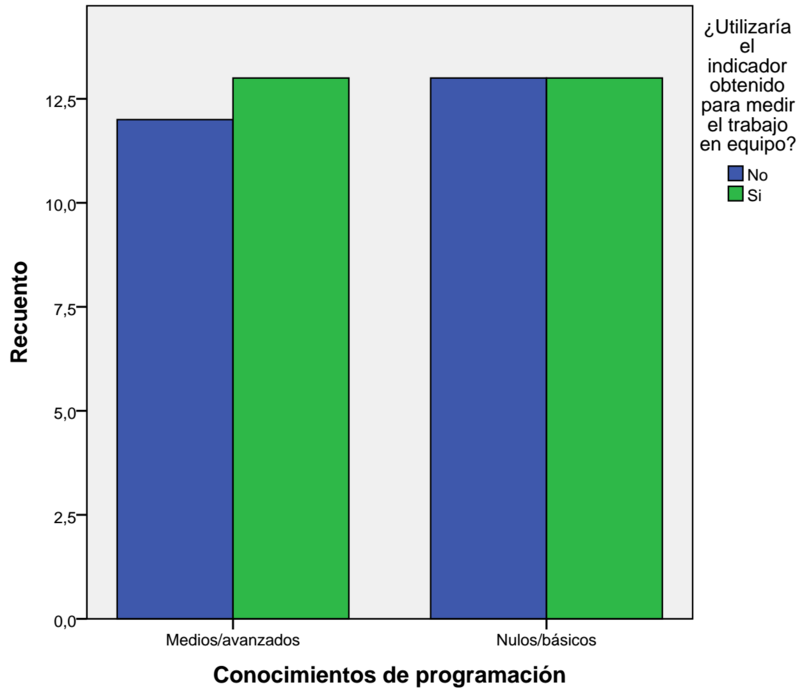
\includegraphics[scale=0.3]{barras_programacion_equipo.png}
  \end{center}
  \caption{Utilizaría el indicador para evaluar el trabajo en equipo}
  \label{fig:app:barras:programacion:equipo}
\end{figure}

Para demostrar la independencia entre los conocimientos de programación y la validez que da el encuestado al indicador para evaluar dicha competencia vamos a definir la siguiente hipótesis nula:

\begin{mdframed}[style=hipotesis0]
$H_0$: \emph{Los \textbf{conocimientos de programación} son independientes de que el individuo considere que les son válidos los indicadores extraídos para medir la competencia de \textbf{trabajo en equipo}}
\end{mdframed}

%Seguir por esta hipotesis ...

En la figura~\ref{fig:app:barras:perfil:equipo} se pueden ver las respuestas de los encuestados a si utilizarían o no el indicador proporcionado para evaluar el trabajo en equipo de los usuarios del wiki en base a su perfil.

\begin{figure}
  \begin{center}
    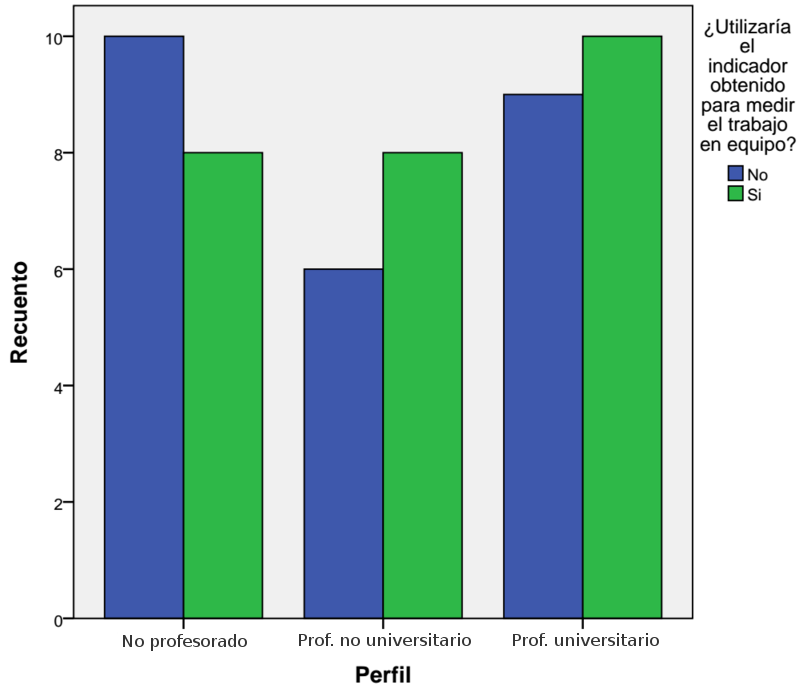
\includegraphics[scale=0.3]{barras_perfil_equipo.png}
  \end{center}
  \caption{Utilizaría el indicador para evaluar el trabajo en equipo}
  \label{fig:app:barras:perfil:equipo}
\end{figure}

Para demostrar la independencia entre los conocimientos de programación y la validez que da el encuestado al indicador para evaluar dicha competencia vamos a definir la siguiente hipótesis nula:

\begin{mdframed}[style=hipotesis0]
$H_0$: \emph{Los \textbf{conocimientos de programación} son independientes de que el individuo considere que les son válidos los indicadores extraídos para medir la competencia de \textbf{planificación y gestión del tiempo}}
\end{mdframed}

\subsection{Planificación y gestión del tiempo}

En la figura~\ref{fig:app:barras:programacion:planificacion} se pueden ver las respuestas de los encuestados a si utilizarían o no el indicador proporcionado para evaluar la planificación y gestión del tiempo de los usuarios del wiki en base a sus conocimientos de programación.

\begin{figure}
  \begin{center}
    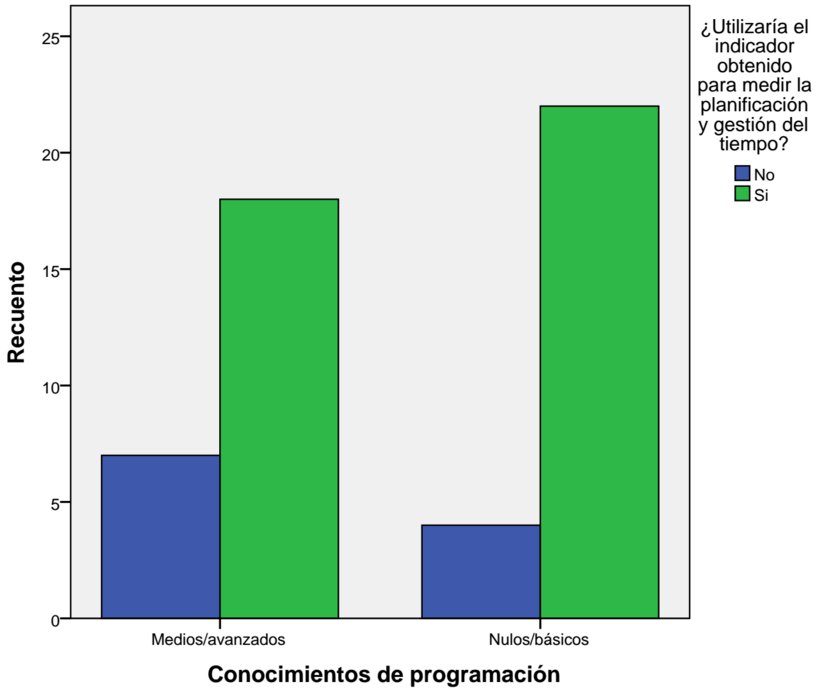
\includegraphics[scale=0.3]{barras_programacion_planificacion.png}
  \end{center}
  \caption{Utilizaría el indicador para evaluar la planificación y gestión de tiempo}
  \label{fig:app:barras:programacion:planificacion}
\end{figure}

Para demostrar la independencia entre los conocimientos de programación y la validez que da el encuestado al indicador para evaluar dicha competencia vamos a definir la siguiente hipótesis nula:

\begin{mdframed}[style=hipotesis0]
$H_0$: \emph{Los \textbf{conocimientos de programación} son independientes de que el individuo considere que les son válidos los indicadores extraídos para medir la competencia de \textbf{liderazgo}}
\end{mdframed}

En la figura~\ref{fig:app:barras:perfil:planificacion} se pueden ver las respuestas de los encuestados a si utilizarían o no el indicador proporcionado para evaluar la planificación y gestión del tiempo de los usuarios del wiki en base a su perfil.

\begin{figure}
  \begin{center}
    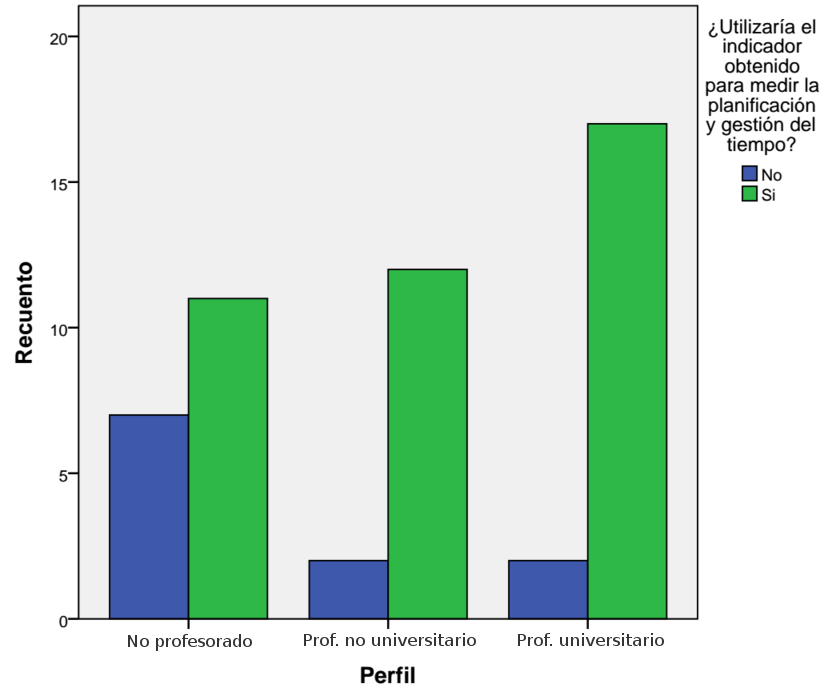
\includegraphics[scale=0.3]{barras_perfil_planificacion.png}
  \end{center}
  \caption{Utilizaría el indicador para evaluar la planificación y gestión de tiempo}
  \label{fig:app:barras:perfil:planificacion}
\end{figure}

Para demostrar la independencia entre los conocimientos de programación y la validez que da el encuestado al indicador para evaluar dicha competencia vamos a definir la siguiente hipótesis nula:

\begin{mdframed}[style=hipotesis0]
$H_0$: \emph{El \textbf{perfil} del individuo es independiente de que el individuo considere que les son válidos los indicadores extraídos para medir la competencia de \textbf{trabajo en equipo}}
\end{mdframed}

\subsection{Liderazgo}

En la figura~\ref{fig:app:barras:programacion:liderazgo} se pueden ver las respuestas de los encuestados a si utilizarían o no el indicador proporcionado para evaluar el liderazgo de los usuarios del wiki en base a sus conocimientos de programación.

\begin{figure}
  \begin{center}
    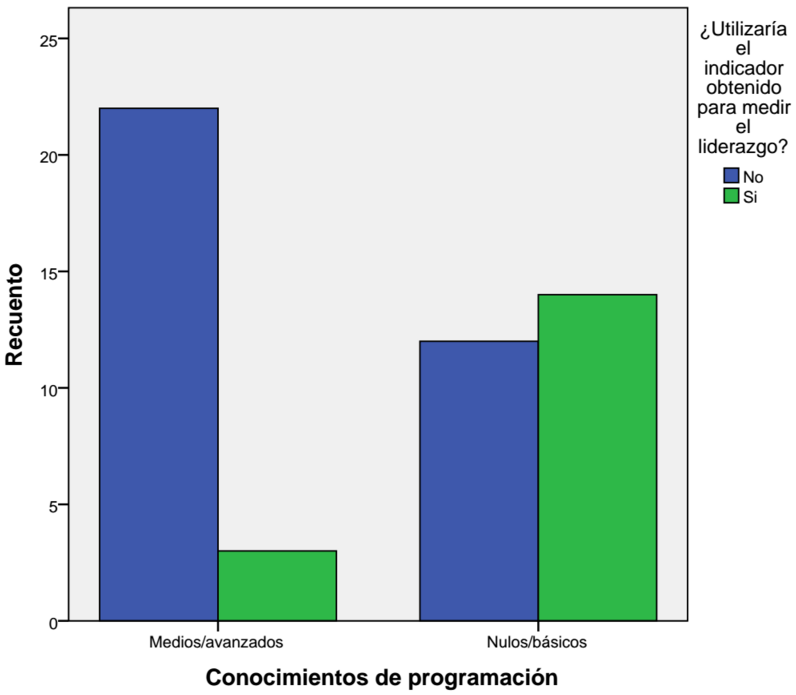
\includegraphics[scale=0.3]{barras_programacion_liderazgo.png}
  \end{center}
  \caption{Utilizaría el indicador para evaluar el liderazgo}
  \label{fig:app:barras:programacion:liderazgo}
\end{figure}

Para demostrar la independencia entre los conocimientos de programación y la validez que da el encuestado al indicador para evaluar dicha competencia vamos a definir la siguiente hipótesis nula:

\begin{mdframed}[style=hipotesis0]
$H_0$: \emph{El \textbf{perfil} del individuo es independiente de que el individuo considere que les son válidos los indicadores extraídos para medir la competencia de \textbf{planificación y gestión del tiempo}}
\end{mdframed}

En la figura~\ref{fig:app:barras:perfil:liderazgo} se pueden ver las respuestas de los encuestados a si utilizarían o no el indicador proporcionado para evaluar el liderazgo de los usuarios del wiki en base a su perfil.

\begin{figure}
  \begin{center}
    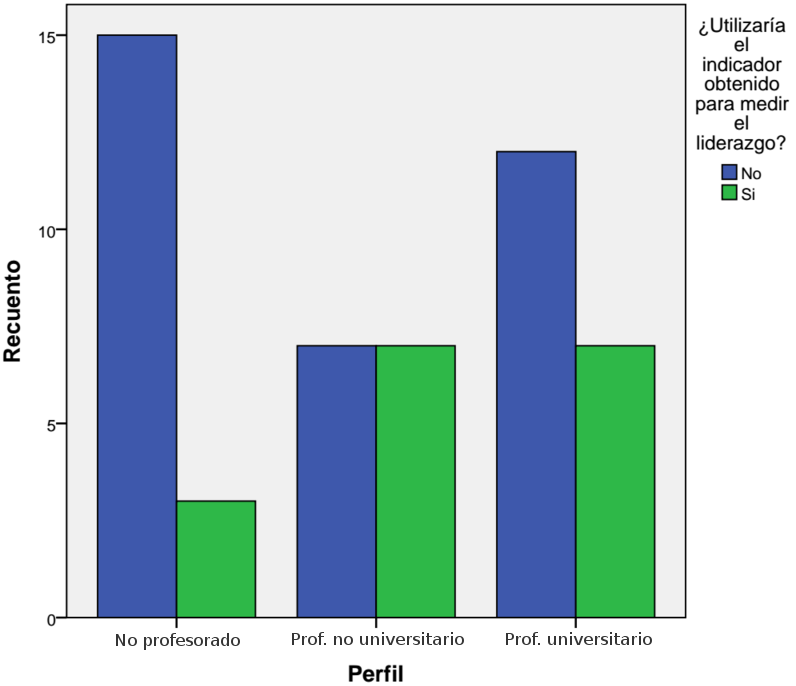
\includegraphics[scale=0.3]{barras_perfil_liderazgo.png}
  \end{center}
  \caption{Utilizaría el indicador para evaluar el liderazgo}
  \label{fig:app:barras:perfil:liderazgo}
\end{figure}

Para demostrar la independencia entre los conocimientos de programación y la validez que da el encuestado al indicador para evaluar dicha competencia vamos a definir la siguiente hipótesis nula:

\begin{mdframed}[style=hipotesis0]
$H_0$: \emph{El \textbf{perfil} del individuo es independiente de que el individuo considere que les son válidos los indicadores extraídos para medir la competencia de \textbf{liderazgo}}
\end{mdframed}


